\documentclass[a4paper,10pt,abstracton,notitlepage]{scrreprt}
\usepackage[utf8]{inputenc}
\usepackage{fullpage}
\usepackage{hyperref}
\usepackage{isomath}
\usepackage{amsfonts}
\usepackage{amsmath}
\usepackage{graphicx}
\usepackage{float}
\usepackage{wrapfig}
\usepackage{caption}
\usepackage[export]{adjustbox}
\usepackage{gnuplottex}


\captionsetup{font={small}}

\title{Dynamic loading of 3D models}
\subtitle{PROJ-H-402 Project Report}
\author{Tim Lenertz, INFO MA1, ULB}
\date{\today}

\begin{document}

\maketitle{}

\vspace{3cm}
\renewcommand{\abstractname}{Résumé}
\begin{abstract}
résumé en français
\end{abstract}

\vspace{2cm}
\renewcommand{\abstractname}{Abstract}
\begin{abstract}
english abstract
\end{abstract}

\tableofcontents{}

\chapter{Introduction}
Point clouds are a way of digitally representing three-dimensional models using only a set of points located on the object's surfaces\footnote{Only non-volumetric point clouds are considered for this project. In volumetric point clouds, points are not only located on surfaces, but on the insides of objects as well.}. Each point consists of 3 coordinates $(x, y, z)$ on an Euclidian coordinate system defined for the model, and can be attributed with additional information such as color, surface normal vector, and others.

This data is typically produced by 3D scanners, which today can capture surfaces at a very high level of detail and thus yield huge quantities of points. Full representations of large objects or environments can be generated by combining the outputs of multiple scans from different view points. For example to get a full point cloud model of an archeological site, aerial scans may be combined with close-up scans of individual landmarks. The resulting files can easily reach several GB in size and contain over $10^{8}$ points, and so they can no longer be processed or visualized efficiently as a whole. Instead, subsets of points around an area of interest are extracted.

The goal of this project is to develop a system which dynamically loads the visible subsets of points to render, while a user moves through a large scale point cloud. This involves methods to extract the right subsets from the point cloud, the data structure which the full point cloud is stored in, and the file format using which this data structure is serialized on secondary storage. The process should appear seamless to the user.

To this end, different data structures and file formats were compared for their possibilities to extract the right subsets of points in an efficient way, and a program was developped which converts a given point cloud file into such a data structure (preprocessing stage), and then allows the user to explore the point cloud, by dynamically loading chunks of it from the preprocessed data structure file.


\chapter{Filtering the point cloud}
This chapter describes the methods used to compute a smaller set of points based on the full point cloud, which visually represent the model as seen from a given view point. The data structure used to store the point cloud is not considered in this chapter.

\section{Definitions}
The following definitions are used throughout this report. A \emph{point cloud} is an unordered set of points with an Euclidian coordinate system. Each \emph{point} $p = \langle x, y, z, r, g, b\rangle$ consists of its coordinates $x, y, z$, and RGB color information. The \emph{model} $P$ is the full point cloud used as input. The \emph{point capacity} $C$ is the maximal number of points that can be outputted to the renderer. 

The \emph{view-projection matrix} $\matrixsym{M} = \matrixsym{P} \times \matrixsym{V}$ is a 4x4 matrix that defines the view frustum of the camera. The 6 planes of the frustum can be derived from the matrix as described in \cite{Gri2001}. The \emph{view matrix} $\matrixsym{V}$ transforms the points' coordinate system into one centered around the camera at its current position and orientation, while the \emph{projection matrix} $\matrixsym{P}$ is used to project the points to their two-dimensional screen coordinates. $\matrixsym{P}$ might define both a parallel projection or a perspective projection with a given \emph{field of view} $\lambda$.

The \emph{filtering function} $f_{P}(\matrixsym{M})$ computes a set of rendered points $P'$ from and model $P$, the matrix $\matrixsym{M}$, and additional parameters. Its main constraint is that $|P'| \leq C$ (whereas $|P|$ may be much larger than $C$). $P'$ does not need to be a subset of $P$: Some methods (such as uniform downsampling) will add points into $P'$ that are not in $P$, in order to achieve a better visual quality.

The criteria for quality of the filtering function is that the 2D projection of $P'$ at the current view point $\matrixsym{M}$ looks similar to that of $P$, that is there should be no loss of important details and no obvious visual artifacts or discontinuities. Techniques such as hidden surface removal can actually improve the appearance of $P'$ compared to that of $P$.

The function $f_{P}$ described in this chapter is an idealized version that operates on a set of points. The next chapters describe algorithms that calculate an approximation of $f_{P}(\matrixsym{M})$ using a specific data structure for $P$, and with additional time complexity constraints.


\section{Projection}
When the point cloud is rendered, the points $p$ are projected from their three-dimensional virtual space onto the two-dimensional screen, using the view frustum defined by $\matrixsym{M}$. This can be described as a function $\mathrm{proj}_{\matrixsym{M}}(x, y, z) = (x_{\mathrm{screen}}, y_{\mathrm{screen}})$, where $x_{\mathrm{screen}} \in [0, w[$ and $y_{\mathrm{screen}} \in [0, h[$, with $w$ and $h$ being the width and height of the screen in pixels. This operation is done on the GPU to render vertices.

First a vector in homogeneous coordinates is build from $x, y, z$: $\overrightarrow{p} = [x, y, z, 1]^{T}$. The fourth component $w = 1$ indicates that this vector represents a point in space; with $w = 0$ it would indicate a direction. In general, a point in homogeneous coordinates $[x, y, z, w]$ corresponds to $[\frac{x}{w}, \frac{y}{w}, \frac{z}{w}]$ in Euclidian coordinates. This allows for building transformation matrices that distinguish between points and vectors (notably for translations), and the projection matrix $\matrixsym{P}$.

Next $\overrightarrow{p}$ is multiplied by $\matrixsym{M}$: $\overrightarrow{p'} = \matrixsym{M} \times \overrightarrow{p} = \matrixsym{P} \times \matrixsym{V} \times \overrightarrow{p}$. The view matrix $\matrixsym{V}$ represents the position and orientation of the camera in the virtual space, so the first multiplication puts $\overrightarrow{p}$ into a coordinate system centered around the camera. The $w$ component remains $1$. It is then multiplied by $\matrixsym{P}$, which can change $w$. Finally the resulting $\overrightarrow{p'}$ is transformed back into Euclidian coordinates to yield the camera coordinates $x_{\mathrm{cam}}, y_{\mathrm{cam}}, z_{\mathrm{cam}}$. In the case of perspective projection, foreshortening is done with the component-wise division by $w$. Because this is a non-affine transformation, it could not be done using matrix arithmetic only.

Camera coordinates are considered to be inside the view frustum only if $x_{\mathrm{cam}}, y_{\mathrm{cam}}, z_{\mathrm{cam}} \in [-1, 1]$, and then the two-dimensional screen coordinates $x_{\mathrm{screen}}, y_{\mathrm{screen}}$ are deduced by linearly mapping $x_{\mathrm{cam}}$ and $y_{\mathrm{cam}}$ to $[0, w[$ and $[0, h[$, respectively. $z_{\mathrm{cam}}$ no longer affects the position of the pixel, but comparing two values for $z_{\mathrm{cam}}$ indicates whether one point is in front of or behind another one in camera space, and is for example used in OpenGL's depth testing.

If $\matrixsym{P}$ is the identity matrix, it represents an orthographic projection where the view frustum is the axis-aligned cube from $[-1, -1, -1]$ to $[1, 1, 1]$. An orthogonal projection with a different cuboid frustum can be expressed by letting $\matrixsym{P}$ be a transformation matrix that maps coordinates in that cuboid to the former cube. The perspective projection matrix for field of view $\lambda$, screen aspect ratio $w/h$, and near and far clipping planes $z_{\mathrm{near}}$ and $z_{\mathrm{far}}$ is defined by:

\begin{displaymath}
\matrixsym{P} = \begin{bmatrix}
\frac{f}{w/h} & 0 & 0 & 0 \\
0 & f & 0 & 0 \\
0 & 0 & \frac{z_{\mathrm{far}} + z_{\mathrm{near}}}{z_{\mathrm{near}} - z_{\mathrm{far}}} & \frac{2 \times z_{\mathrm{far}} \times z_{\mathrm{near}}}{z_{\mathrm{near}} - z_{\mathrm{far}}} \\
0 & 0 & -1 & 0
\end{bmatrix}
\text{ with }
f = \frac{1}{\tan(\frac{\lambda}{2})}
\end{displaymath}


\section{Frustum culling}
The simplest and most effective filtering done by $f_{P}$ is \emph{view frustum culling}, which removes all points from $P$ that are not within the view frustum defined by $\matrixsym{M}$. This usually eliminates more than half of the points from the model: Those behind the viewer, those outside his field of view, and those too far away (beyond the far clipping plane $z_{\mathrm{far}}$). It is done implicitly by the GPU, but the goal of the filtering is to reduce the number of points before they are sent to the GPU.

Frustum culling can be done per point by clipping the camera coordinates as described above, but depending on the data structure used, entire regions of the model space will be tested to be inside or outside the frustum instead.


\section{Downsampling}
Downsampling reduces the density of points. Because of foreshortening in perspective projection, sections of the model that are farther away from the camera will become smaller in the two-dimensional projection, and as a consequence their amount and density of points increases. Since a smaller density is sufficient to visually represent the model, it makes sense to apply downsampling on regions of the point cloud, depending on their distance from the camera.

Because the point cloud is non-volumetric, points are distributed on two-dimensional surfaces of the three-dimensional model. So the density can be defined as the number of points per surface area $\rho = n/A$. Because of the way the point clouds are generated, $\rho$ will remain approximately constant on small scale, but on composite point clouds that combine different scans, $\rho$ can vary greatly in different regions of the point cloud. Some objects could have been scanned close-up, while the surrounding environment has a much lower resolution. 

The level of downsampling is determined by a function $r(d)$ which gives a ratio in function of a distance to the camera. A downsampling algorithm will transform the point cloud such that at any surface position $\overrightarrow{p}$, the density becomes $\rho' = r(d(\overrightarrow{p})) \times \rho$ (with $r \in [0, 1]$). The algorithms used here operate without knowledge of the shape of the object's surface or of the concrete value of $\rho$.

\subsection{Weighted points}
One method of doing downsampling is to assign a weight $w \in [0, 1]$ to each point $p \in P$, and let the downsampled set of points be the subset $P' = \{ p \in P : w(p) < r(d(p)) \}$. For this to work the weights $w$ need to be uniformly distributed among the points.

This leads to a continuous $\rho'$, so no visual discontinuities are produced. Also, if the data structure contains the weighted points $P$ in a list ordered by ascending $w$, then it is possible to dynamically extract $P'$ in time $O(|P'|)$.

\begin{wrapfigure}{r}{7cm}
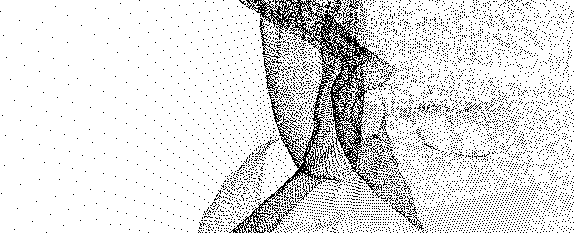
\includegraphics[width=7cm,frame]{random_weights_inv.png}
\caption{Weighted points downsampling using random weights}
\label{fig:random_weights}
\end{wrapfigure}
A simple way to define the weights is to set each weight to a random value. However, this leads to an irregular pattern in the way downsampled points are placed on the surface, as seen in figure \ref{fig:random_weights}. The left-hand side of the point cloud is not downsampled and retains a more regular pattern.

\subsection{LOD regions}
Another possibility is to first compute several downsampled point sets $P'_{r}$ with fixed downsampling ratios $r$, during preprocessing. $P'(\overrightarrow{p})$ is then produced out of pieces of these sets, by choosing the set whose value $r$ is closest to $r(d(\overrightarrow{p})$. The resulting $P'$ is thus composed of several \emph{level of detail} (LOD) regions\footnote{These are called \emph{mipmaps} in the implementation}, so $\rho'(d)$ becomes a non-continuous staircase function, and visual discontinuities are produced. However, this method allows for producing the sets $P'_{r}$ with no time constraints and with a constant $r$.

In figure \ref{fig:uniform_example}, the region farther away was downsampled this way (using uniform downsampling). A visual discontinuity can be seen in the lower-right corner.

\subsection{Uniform downsampling}
Uniform downsampling is a downsampling algorithm that aims to produce a more regular pattern in the distribution of points on $P'$, as opposed to that produced by random downsampling (figure \ref{fig:random_weights}). It operates using a constant ratio $r$.

\begin{wrapfigure}{r}{7cm}
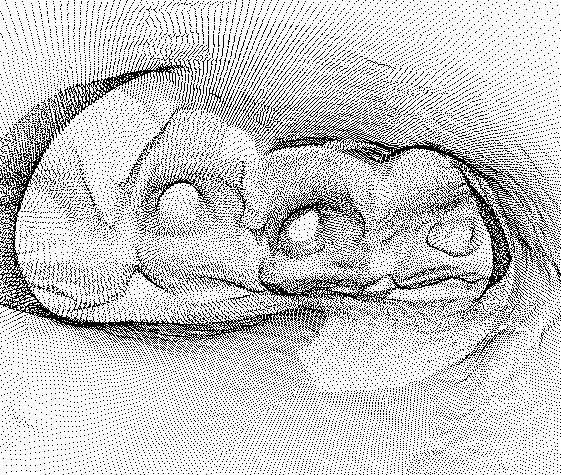
\includegraphics[width=7cm,frame]{uniform_example_inv.png}
\caption{Example of uniform downsampling}
\label{fig:uniform_example}
\end{wrapfigure}
The input point set $P$ is divided into a regular grid of cubes $C_{i,j,k}$ with side length $s$. For all cubes that contain at least one point, exactly one single point $p'$ is outputted into $P'$, whose position is the mean of that of the points in $C$, and whose color is that of the point $p \in P$ closest to that position. Figure \ref{fig:uniform_algo} illustrates the procedure in two dimensions. The more regular aspect of $P'$ is because its points are constrained by the regular grid. The algorithm also does not require $P$ to have a regular pattern to begin with.

The main difficulty is to find the value for the side length $s$, such that $n = |P'|$ is approximately equal to $r \times |P|$. Figure \ref{fig:uniform_stat} shows how $n$ varies in function of $s$ for some example models: In general, $n$ gets larger as the side length $s$ gets smaller, because there are more cubes available in the region of the model. Because the cubes are non-overlapping and each point $p \in P$ belongs to exactly one cube, $n$ is at most $|P|$. It reaches this value once $s$ gets reaches a value (depending on the density) where each point belongs to a different cube.

However, the function is not entirely monotonic, as the close-up view in figure \ref{fig:uniform_stat_detail} shows. This is because when $s$ gets changes, all cubes on the grid (except those at the origin) get displaced. So it is possible that two neighboring points fit into one cube for one value of $s$, but for $s' > s$ the grid becomes such that a boundary lies between these points. This effect only occurs at the small scale because as $s$ gets even larger, the boundary moves further so the two points again fit into one cube, and many more points in the model fit into the same cubes.

Because the points are not distributed evenly in space but rather on the object's surfaces, but the algorithm operates in three-dimensional space, there is way to effectively estimate a value for $n(s)$. Instead the algorithm does a dichotomic search to find a value $s$ such that $n \approx r \times |P|$, within a certain tolerance. The small-scale ascending intervals of $s(n)$ are taken into account.

\begin{figure}[p]
\centering
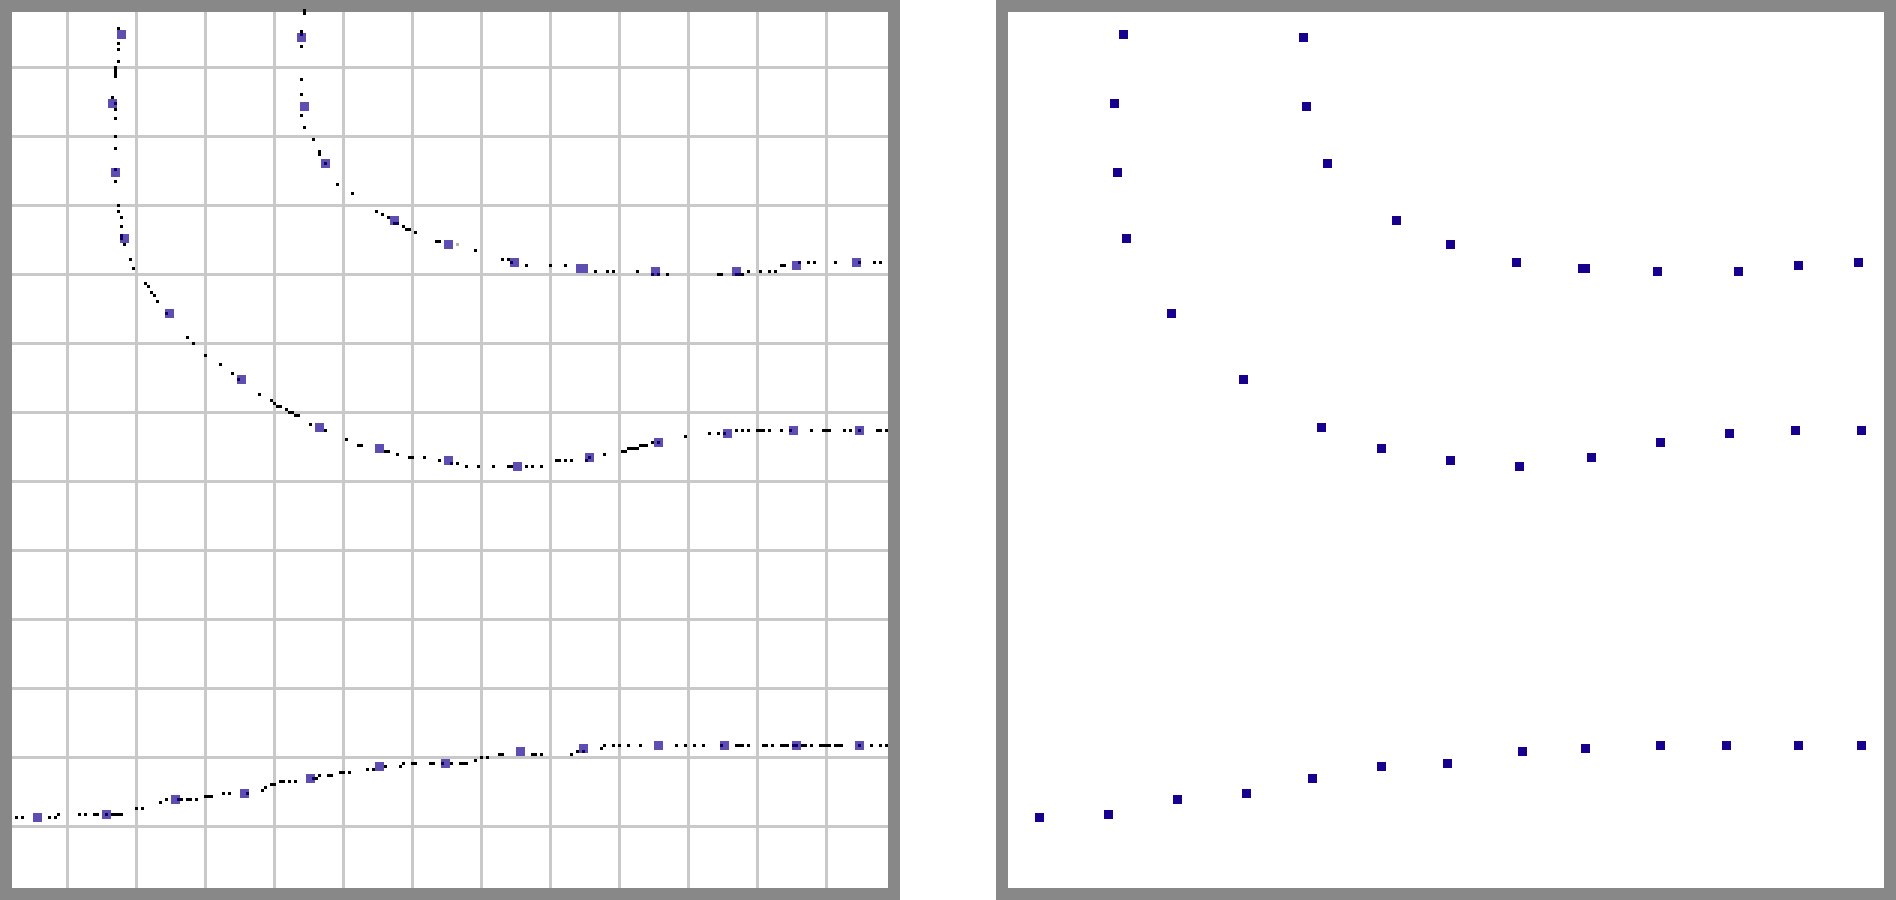
\includegraphics[width=7cm]{uniform.png}
\caption{Two-dimensional visualization of uniform downsampling algorithm}
\label{fig:uniform_algo}
\end{figure}

\begin{figure}[p]
\centering
\begin{gnuplot}
	set terminal epslatex color
	set xlabel "$s$"
	set ylabel "$n / |P|$"
	plot \
		"stat\_dragon.dat" using 1:($2/3609599+0*$2) smooth unique linetype rgb "black" title "dragon.ply", \
		"stat\_statuette.dat" using 1:($2/4999995+0*$2) smooth unique linetype rgb "red" title "statuette.ply", \
		"stat\_scan.dat" using 1:($2/681124+0*$2) smooth unique linetype rgb "blue" title "scan.ply"
\end{gnuplot}
\caption{Number of output points $n$ VS cubes side length $s$ in uniform downsampling; normalized by number of points in model $|P|$}
\label{fig:uniform_stat}
\end{figure}

\begin{figure}[p]
\centering
\begin{gnuplot}
	unset key
	set ylabel "$n$"
	set xlabel "$s$"
	plot "uniform\_stat\_detail.dat" smooth unique
\end{gnuplot}
\caption{Close-up view of figure \ref{fig:uniform_stat}}
\label{fig:uniform_stat_detail}
\end{figure}


\subsection{Choosing the downsampling ratio}
The function $r(d)$ determines that ratio of downsampling that should be applied depending on the distance $d$ to the camera. If \emph{LOD regions} are used, it is a staircase function and can only take a small number of different values, otherwise (\emph{weighted points}) it is continuous.

Let $L$ be the number of \emph{LOD regions} (``levels''). In the program, it is usually 1, 4, 8 or 16. For \emph{weighted points} downsampling, $L$ can take any value and can be changed at runtime. In both cases, $r(d)$ is defined the same way:

$r_{\ell}(\ell, a, L, n, n_{\min})$ gives the downsampling ratio for level $\ell \in [0, L-1]$. $n$ is the total number of points used as input to the downsampling algorithm, $n_{\min}$ the minimal number of points the should be outputted. If the algorithm is applied to the full model $n = |P|$ (number of points in model), and $n_{\min} = C$ (capacity of renderer) is used, since the goal is to stay as close as possible but inferior to $C$, so as to not lose more points than necessary. The function is defined such that $r_{\ell}(\ell = 0) = n$ (level 0 means no downsampling), $r_{\ell}(\ell = L-1) = n_{min}$ (maximal possible downsampling must be reached on last level), and it is stictly decreasing. The \emph{amount} parameter $a$ sets how strongly the function should be decreasing, and must be adjusted to fit the input model.

If \emph{LOD regions} are used, this function is evaluated in the preprocessing stage, when the $L-1$ downsampled point sets are created. For \emph{weighted points}, it is evaluated at runtime. Then, $a$ and $L$ also can be changed at runtime, and $\ell$ can take real values (as opposed to integers only). This allows for continuous downsampling.

The level to use at a given location is chosen by the function $\ell(d, s)$, where $d$ is the distance to the cemera, and the \emph{setting} $s$ a parameter that can always be adjusted at runtime (unlike $a$). The function is defined such that $\ell(d = 0) = 1$ (no downsampling when very close to camera), and $\lim_{d \rightarrow \infty} = L$ (eventually reach maximal level). Also, it increases with $d$, where $s$ determines how quickly. $\ell(d, s)$ is defined as a real function, but when \emph{LOD regions} are used, the floor value $\lfloor \ell(d, s) \rfloor$ is always taken.

In short, the process of choosing the downsampling ratio $r(d)$ in function of distance $d$ works as follows: For \emph{weighted points}, $r(d) = r_{\ell}(\ell(d, s), a, L, n, n_{min})$ is evaluated at runtime, and $s, a, L$ can all be adjusted at runtime. Thus $r(d)$ is continuous.

For \emph{LOD regions}, $L$ point sets are created in the preprocessing stage which are downsampled with ratio $r_{ell}(i, a, L, n, n_{min})$. The integer $i \in 0 \hdots L-1$ is the level of the point set, and $a, L, n, n_{min}$ all need to be known in this stage. The program stores the downsampling ratios associated with the $L$ levels with the generated data structure. At runtime, the downsampled point set for level $i = \lfloor \ell(d, s) \rfloor$ is chosen depending on $d$. Only $s$ can be adjusted at runtime.

\subsection{Definition of the downsampling functions}
The functions $\ell$ and $r_{\ell}$ are defined as follows:
\begin{displaymath}
	\ell(d, s) = \begin{cases}
		\min \{ \frac{d - d_{0}}{\Delta d}, L-1 \} & d > d_{0} \\
		0 & d \leq d_{0}
	\end{cases}
\end{displaymath}

with $d_{0} = s^{e}$ the \emph{start distance}, i.e. the distance from the camera where downsampling should start, and $\Delta d = s$ the \emph{step distance} after which the next level is chosen.

So the level is chosen linearily with the distance, with an offset $d_{0}$. The \emph{setting} $s$ controls the intervals between levels and the start distance. In the program, the $e$ is fixed to the value $e = 1.3$. It makes sure that $d_{0}$ scales faster than linearily with $s$, because the jump from no downsampling to the first level of downsampling represents a greater loss in output quality than the jump between downsampling levels.

The following graph shows the function in its staircase form, with different values for $s$.

\begin{figure}[H]
\centering
\begin{gnuplot}
	set terminal epslatex color
	set ylabel "level"
	set xlabel "$d$"
	set ytics (0, 1, 2, 3, 4, 5, 6, 7, 8, 9, 10, 11, 12, 13, 14, 15)

	levels = 16
	xp = 1.3
	maxd = 700

	set xrange [0:maxd]
	set yrange [0:levels + 3]
	unset autoscale

	start_distance(s) = s**xp
	step_distance(s) = s
	constrain_lvl(l) = (l > levels - 1) ? (levels - 1) : l

	l(d, s) = constrain_lvl( \
		(d > start_distance(s)) ? ((d - start_distance(s)) / step_distance(s)) : 0 \
	)
	
	plot [d=0:maxd] \
		floor(l(d, 20)) with steps lt rgb "black" title "$s = 20$", \
		floor(l(d, 10)) with steps lt rgb "blue" title "$s = 10$", \
		floor(l(d, 50)) with steps lt rgb "red" title "$s = 50$"
\end{gnuplot}
\caption{Downsampling level for distance function $\ell(d, s)$}
\label{fig:downsampling_ell_d}
\end{figure}


The downsampling ratio function is defined as follows:
\begin{displaymath}
	r_{\ell}(\ell, a, L, n, n_{\min}) = 1 - (1 - r_{\min}) \left( \frac{\ell}{L-1} \right)^{a}
\end{displaymath}
where $r_{min} = \max \{ \frac{n_{\min}}{n}, 1 \}$ is the minimal downsampling ratio. Note that when $n \leq n_{min}$, the function always yields $1$ and no downsampling will be applied. 

The following graph shows the function with different values for the downsampling amount $a$:

\begin{figure}[H]
\centering
\begin{gnuplot}
	set terminal epslatex color
	set ylabel "$r$"
	set xlabel "level"
	set xtics (0, 1, 2, 3, 4, 5, 6, 7, 8, 9, 10, 11, 12, 13, 14, 15)

	n = 5000000
	nmin = 1000000
	rmin = nmin / n
	levels = 16

	set xrange [0:(levels - 1)]
	set yrange [0:1]
	unset autoscale
	
	r(l, a) = 1 - (1 - rmin) * (l/(levels - 1))**a
	plot [l=0:(levels - 1)] \
		r(l, 2) lt rgb "black" title "$a = 2.0$", \
		r(l, 1.2) lt rgb "blue" title "$a = 1.2$", \
		r(l, 0.4) lt rgb "green" title "$a = 0.4$", \
		r(l, 3.8) lt rgb "red" title "$a = 3.8$"
\end{gnuplot}
\caption{Downsampling ratio for level function $r_{\ell}(d, a)$}
\label{fig:downsampling_r_ell}
\end{figure}

\begin{wrapfigure}{r}{7cm}
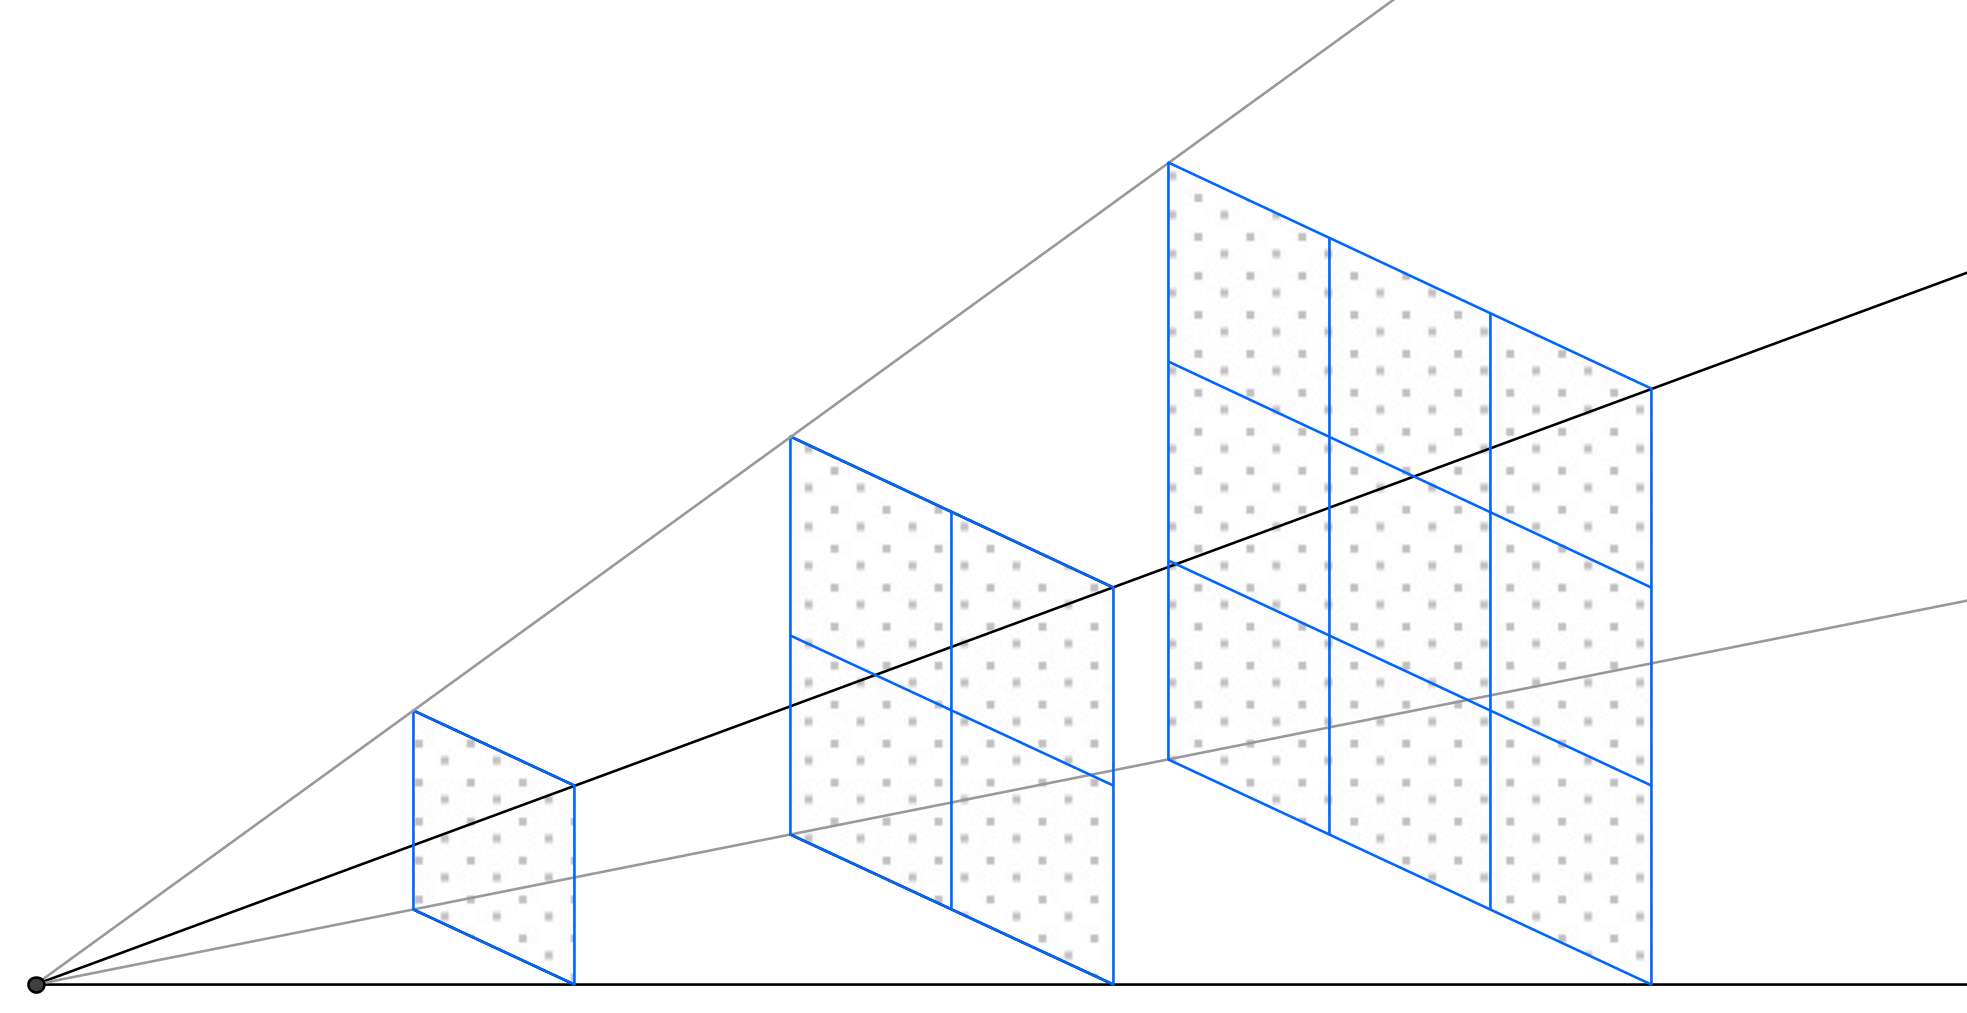
\includegraphics[width=7cm]{distanceDensity.png}
\caption{Perspective projection and area}
\label{fig:distance_density}
\end{wrapfigure}
Figure \ref{fig:distance_density} shows visible areas\footnote{In reality, the areas would be curved (intersection of view frustum and sphere of radius $d$), but the simplification holds because the field of view is small} with distances $d$, $2d$ and $3d$ to the camera in a perspective projection. Their area is proportional to $d^{2}$. Supposing that surfaces of the point cloud is located exactly on these areas, the point density of the projection $\rho'$ would also be proportional to $d^{2}$.

Since $\rho'$ should be more or less constant, setting $a = 2$ makes sense as it cancels out the effect. In practice, it needs to be adjusted to fit the particular point cloud.

Finally, this graph shows $r_{d, s}$ ($r_{\ell} \circ \ell$) in piecewise form, with $a = 2$, $L = 16$ and $r_{\min} = 0.2$:

\begin{figure}[H]
\centering
\begin{gnuplot}
	set terminal epslatex color
	set ylabel "$r$"
	set xlabel "$d$"

	levels = 16
	xp = 1.3
	maxd = 800
	n = 5000000
	nmin = 1000000
	rmin = nmin / n
	a = 2


	start_distance(s) = s**xp
	step_distance(s) = s
	constrain_lvl(l) = (l > levels - 1) ? (levels - 1) : l

	r(l) = 1 - (1 - rmin) * (l/(levels - 1))**a

	l(d, s) = constrain_lvl( \
		(d > start_distance(s)) ? ((d - start_distance(s)) / step_distance(s)) : 0 \
	)
	
	rd(d, s) = r( 0.0 + floor( l(d, s) ) )
	rdc(d, s) = r( 0.0 + l(d, s) )
	
	plot [d=0:maxd] \
		rd(d, 20) with steps lt rgb "black" title "$s = 20$", \
		rd(d, 10) with steps lt rgb "blue" title "$s = 10$", \
		rd(d, 50) with steps lt rgb "red" title "$s = 50$"
\end{gnuplot}
\caption{Downsampling ratio for distance $r(d, s)$}
\label{fig:downsampling_r}
\end{figure}

\subsection{Adaptive downsampling}

\section{Occlusion culling}


\chapter{Data structures}

\section{Cubes structure}
\section{Tree structures}
\subsection{Octree}
\subsection{KdTree}

\chapter{Application}

\chapter{Results}

\chapter{Conclusion}

\bibliographystyle{plain}
\bibliography{report}


\end{document}
